\documentclass[border=12pt]{standalone}
\usepackage{tikz}
\usetikzlibrary{shapes.geometric, arrows.meta, positioning, calc, fit, backgrounds}
\usepackage{fontspec}
\usepackage{amsmath,amssymb}
\setmainfont{DejaVu Sans}

\begin{document}
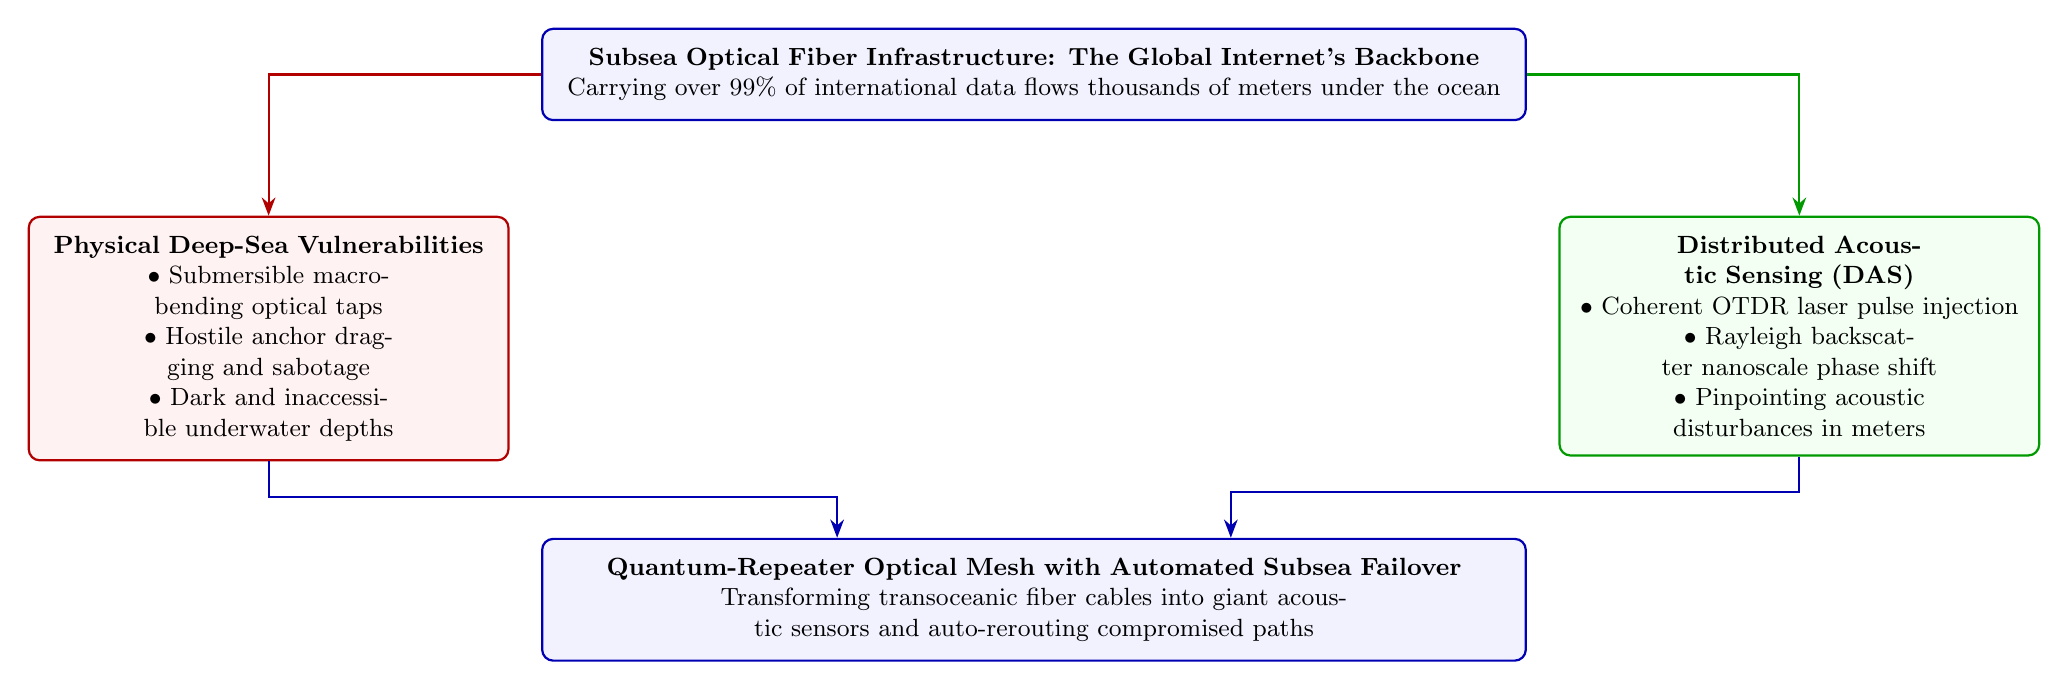
\begin{tikzpicture}[
    font=\small,
    >=Stealth,
    node distance=1.2cm,
    block/.style={rectangle, draw=blue!70!black, fill=blue!5, rounded corners=4pt, thick, align=center, inner sep=7pt},
    alertblock/.style={rectangle, draw=red!70!black, fill=red!5, rounded corners=4pt, thick, align=center, inner sep=7pt},
    greenblock/.style={rectangle, draw=green!60!black, fill=green!5, rounded corners=4pt, thick, align=center, inner sep=7pt},
    amberblock/.style={rectangle, draw=orange!80!black, fill=orange!5, rounded corners=4pt, thick, align=center, inner sep=7pt}
]

\node[block, text width=12cm] (top) {\textbf{Subsea Optical Fiber Infrastructure: The Global Internet's Backbone}\\Carrying over 99\% of international data flows thousands of meters under the ocean};

\node[alertblock, below left=1.2cm and 0.4cm of top, text width=5.6cm] (threat) {\textbf{Physical Deep-Sea Vulnerabilities}\\$\bullet$ Submersible macro-bending optical taps\\$\bullet$ Hostile anchor dragging and sabotage\\$\bullet$ Dark and inaccessible underwater depths};

\node[greenblock, below right=1.2cm and 0.4cm of top, text width=5.6cm] (das) {\textbf{Distributed Acoustic Sensing (DAS)}\\$\bullet$ Coherent OTDR laser pulse injection\\$\bullet$ Rayleigh backscatter nanoscale phase shift\\$\bullet$ Pinpointing acoustic disturbances in meters};

\node[block, below=1.0cm of $(threat.south)!0.5!(das.south)$, text width=12cm] (bottom) {\textbf{Quantum-Repeater Optical Mesh with Automated Subsea Failover}\\Transforming transoceanic fiber cables into giant acoustic sensors and auto-rerouting compromised paths};

\draw[->, thick, red!70!black] (top) -| (threat);
\draw[->, thick, green!60!black] (top) -| (das);
\draw[->, thick, blue!70!black] (threat.south) -- ++(0,-0.45) -| ([xshift=-2.5cm]bottom.north);
\draw[->, thick, blue!70!black] (das.south) -- ++(0,-0.45) -| ([xshift=2.5cm]bottom.north);

\end{tikzpicture}
\end{document}
